%particles
\newcommand{\jpsi}{\rm J/$\psi$}
\newcommand{\psip}{$\psi^\prime$}
\newcommand{\jpsiDY}{\rm J/$\psi$\,/\,DY}
\newcommand{\chic}{$\chi_{\rm c}$}
\newcommand{\pip}{$\pi^{+}$}
\newcommand{\pim}{$\pi^{-}$}
\newcommand{\pizero}{$\pi^{0}$}
\newcommand{\kap}{K$^{+}$}
\newcommand{\kam}{K$^{-}$}
\newcommand{\pbar}{$\rm\overline{p}$}
\newcommand{\ccbar}{\ensuremath{\mathrm{c\overline{c}}}}
\newcommand{\bbbar}{\ensuremath{\mathrm{b\overline{b}}}}
\newcommand{\Dzero}{\ensuremath{\mathrm{D^{0}}}}
\newcommand{\Dzerobar}{\ensuremath{\mathrm{\overline{D}^{0}}}}
\newcommand{\Dpm}{\ensuremath{\mathrm{D^{\pm}}}}
\newcommand{\Ds}{\ensuremath{\mathrm{D_{s}^{\pm}}}}
\newcommand{\Dstar}{\ensuremath{\mathrm{D^{*\pm}}}}

%collision systems
\newcommand{\pp}{pp}
\newcommand{\pPb}{p--Pb}
\newcommand{\PbPb}{Pb--Pb}

%detectors
\newcommand{\ezdc}{$E_{\rm ZDC}$}

%units
\newcommand{\GeVc}{GeV/$c$}
\newcommand{\GeVcsq}{GeV/$c^2$}

%others
\newcommand{\degree}{$^{\rm o}$}
\newcommand{\s}{\ensuremath{\sqrt{s}}}
\newcommand{\snn}{\ensuremath{\sqrt{s_{\rm NN}}}}
\newcommand{\y}{\ensuremath{y}}
\newcommand{\pt}{\ensuremath{p_{\rm T}}}
\newcommand{\dedx}{d$E$/d$x$}
\newcommand{\dndy}{d$N$/d$y$}
\newcommand{\dndydpt}{${\rm d}^2N/({\rm d}y {\rm d}p_{\rm t})$}
\newcommand{\zpar}{\ensuremath{z_{||}}}
\newcommand{\zpargen}{\ensuremath{z_{||}^{\mathrm{part}}}}
\newcommand{\zpardet}{\ensuremath{z_{||}^{\mathrm{det}}}}
\newcommand{\ptchjet}{\ensuremath{p_{\mathrm{T,ch\, jet}}}}
\newcommand{\ptjet}{\ensuremath{p_{\mathrm{T,jet}}}}
\newcommand{\ptchjetgen}{\ensuremath{p_{\mathrm{T,ch\,jet}}^{\mathrm{part}}}}
\newcommand{\ptchjetdet}{\ensuremath{p_{\mathrm{T,ch\,jet}}^{\mathrm{det}}}}
\newcommand{\ptd}{\ensuremath{p_{\mathrm{T,D}}}}
\newcommand{\ptdgen}{\ensuremath{p_{\mathrm{T,D}}^{\mathrm{part}}}}
\newcommand{\ptddet}{\ensuremath{p_{\mathrm{T,D}}^{\mathrm{det}}}}
\newcommand{\antikt}{anti-\ensuremath{k_{\mathrm{T}}}}
\newcommand{\Antikt}{Anti-\ensuremath{k_{\mathrm{T}}}}
\newcommand{\kt}{\ensuremath{k_{\mathrm{T}}}}
\newcommand{\pthard}{\ensuremath{p_{\mathrm{T,hard}}}}

\PassOptionsToPackage{usenames,dvipsnames}{xcolor}
\documentclass{tikzposter}
\tikzposterlatexaffectionproofoff
\usepackage{xcolor}
\usetikzlibrary{positioning}
\usetheme{Rays}

\usepackage{url}
\usepackage{adjustbox}
\usepackage{comment}
\usepackage{overpic}
\usepackage{mathtools}

\makeatletter
\def\title#1{\gdef\@title{\scalebox{\TP@titletextscale}{%
\begin{minipage}[t]{\linewidth}
\centering
#1
\par
\vspace{0.5em}
\end{minipage}%
}}}
\makeatother

\settitle{ \centering \vbox{
     \@titlegraphic \\[\TP@titlegraphictotitledistance] \centering
     \color{titlefgcolor} {\bfseries \Huge \@title \par}
     \vspace*{1em}
     {\huge \@author \par} \vspace*{1em} {\LARGE \@institute}
}}

\title{Exploring the charm content of jets
in \pp\ collisions with ALICE}
\author{Salvatore Aiola, on behalf of the ALICE Collaboration}
\institute{Yale University\\[0.01cm] \url{salvatore.aiola@yale.edu}\\[1cm] 
\begin{minipage}[t]{0.19\linewidth}
\hspace{1cm}
\end{minipage}
%
\begin{adjustbox}{valign=c}
\begin{minipage}[t]{0.1\linewidth}

\includegraphics[width=\linewidth]{img/qm17}
\end{minipage}
\end{adjustbox}
%
\begin{adjustbox}{valign=c}
\begin{minipage}[t]{0.5\linewidth}
February 6-11, 2017, Chicago, IL, USA
\end{minipage}
\end{adjustbox}
%
\begin{minipage}[t]{0.2\linewidth}
\hspace{1cm}
\end{minipage}
}
\makeatletter
\newcommand\insertlogoi[2][]{\def\@insertlogoi{\includegraphics[#1]{#2}}}
\newcommand\insertlogoii[2][]{\def\@insertlogoii{\includegraphics[#1]{#2}}}
\newcommand\insertlogoiii[2][]{\def\@insertlogoiii{\includegraphics[#1]{#2}}}
\newcommand\insertlogoiv[2][]{\def\@insertlogoiv{\hspace{150pt}\includegraphics[#1]{#2}}}
\newlength\LogoSep
\setlength\LogoSep{-150pt}

\insertlogoi[width=4.5cm]{img/yale}
\insertlogoii[width=5cm]{img/yale_text}
\insertlogoiii[width=6.5cm]{img/alice}
\insertlogoiv[width=11cm]{img/doe}

\renewcommand\maketitle[1][]{  % #1 keys
    \normalsize
    \setkeys{title}{#1}
    % Title dummy to get title height
    \node[transparent,inner sep=\TP@titleinnersep, line width=\TP@titlelinewidth, anchor=north, minimum width=\TP@visibletextwidth-2\TP@titleinnersep]
        (TP@title) at ($(0, 0.5\textheight-\TP@titletotopverticalspace)$) {\parbox{\TP@titlewidth-2\TP@titleinnersep}{\TP@maketitle}};
    \draw let \p1 = ($(TP@title.north)-(TP@title.south)$) in node {
        \setlength{\TP@titleheight}{\y1}
        \setlength{\titleheight}{\y1}
        \global\TP@titleheight=\TP@titleheight
        \global\titleheight=\titleheight
    };

    % Compute title position
    \setlength{\titleposleft}{-0.5\titlewidth}
    \setlength{\titleposright}{\titleposleft+\titlewidth}
    \setlength{\titlepostop}{0.5\textheight-\TP@titletotopverticalspace}
    \setlength{\titleposbottom}{\titlepostop-\titleheight}

    % Title style (background)
    \TP@titlestyle

    % Title node
    \node[inner sep=\TP@titleinnersep, line width=\TP@titlelinewidth, anchor=north, minimum width=\TP@visibletextwidth-2\TP@titleinnersep]
        at (0,0.5\textheight-\TP@titletotopverticalspace)
        (title)
        {\parbox{\TP@titlewidth-2\TP@titleinnersep}{\TP@maketitle}};

    \node[inner sep=0pt,anchor=west] 
    (logo_yale_shield)
      at ([shift={(-\LogoSep,-0.8cm)}]title.west)
      {\@insertlogoi};
      
    \node[inner sep=0pt,anchor=west,right=of logo_yale_shield] 
        (logo_yale)
      %at ([xshift=\LogoSep]title.east)
      {\@insertlogoii};

    \node[inner sep=0pt,anchor=east] 
        (logo_alice)
      at ([shift={(\LogoSep,-1.8cm)}]title.east)
      {\@insertlogoiii};
      
    \node[inner sep=0pt,anchor=west,below=of logo_yale_shield] 
        (logo_doe)
      %at ([xshift=\LogoSep]title.east)
      {\@insertlogoiv};

    % Settings for blocks
    \normalsize
    \setlength{\TP@blocktop}{\titleposbottom-\TP@titletoblockverticalspace}
}
\makeatother

\definecolor{darkestblue}{RGB}{1,8,100}
\definecolor{darkerblue}{RGB}{3,17,150}
\definecolor{darkblue}{RGB}{7,26,200}
\definecolor{lightred}{RGB}{202,103,104}
\definecolor{lightgreen}{RGB}{106,202,107}

\begin{document}

\maketitle[width=.9\textwidth]

\begin{columns}

\column{.45}
\block{Introduction}{
\begin{adjustbox}{valign=t}
\begin{minipage}[t]{0.37\colwidth}
\vspace{-20pt}
\begin{tikzfigure}[Prompt \Dzero\ cross section.\par]
     \label{fig:D0mesons}
\begin{overpic}[width=\linewidth, trim=0 0 0 0, clip]{img/D0mesons}
 \put (17,23) {{\scalebox{.5}{Phys.Rev. C94 (2016) 054908}}}
\end{overpic}
 \end{tikzfigure}
\end{minipage}
\end{adjustbox}
%
\begin{adjustbox}{valign=t}
\begin{minipage}[t]{0.56\colwidth}
\textcolor{BrickRed}{\textbf{\Dzero\ mesons measured down to $\ptd\approx0$ in \pp\ and \pPb\ collisions}}
\begin{itemize}
\item Test \textbf{pQCD} at its limits of applicability \\$Q^{2} \approx m_{\rm c}^{2} \approx 1$~\GeVcsq
\item Serves as baseline for \textbf{QGP} measurements
\end{itemize}
\textcolor{ForestGreen}{\textbf{Jet observables are closer to the parton\\ kinematics than single particles}}
\begin{itemize}
\item Measurement of the c quark \textbf{fragmentation}
\item Better sensitivity for the \textbf{dead-cone effect} in the QGP
\end{itemize}
\end{minipage}
\end{adjustbox}
}

\column{.55}
\block{ALICE at the LHC}{
\begin{minipage}[t]{0.34\colwidth}
\begin{tikzfigure}[3D schematics of the ALICE detetcor.\par]
     \label{fig:D0mesons}
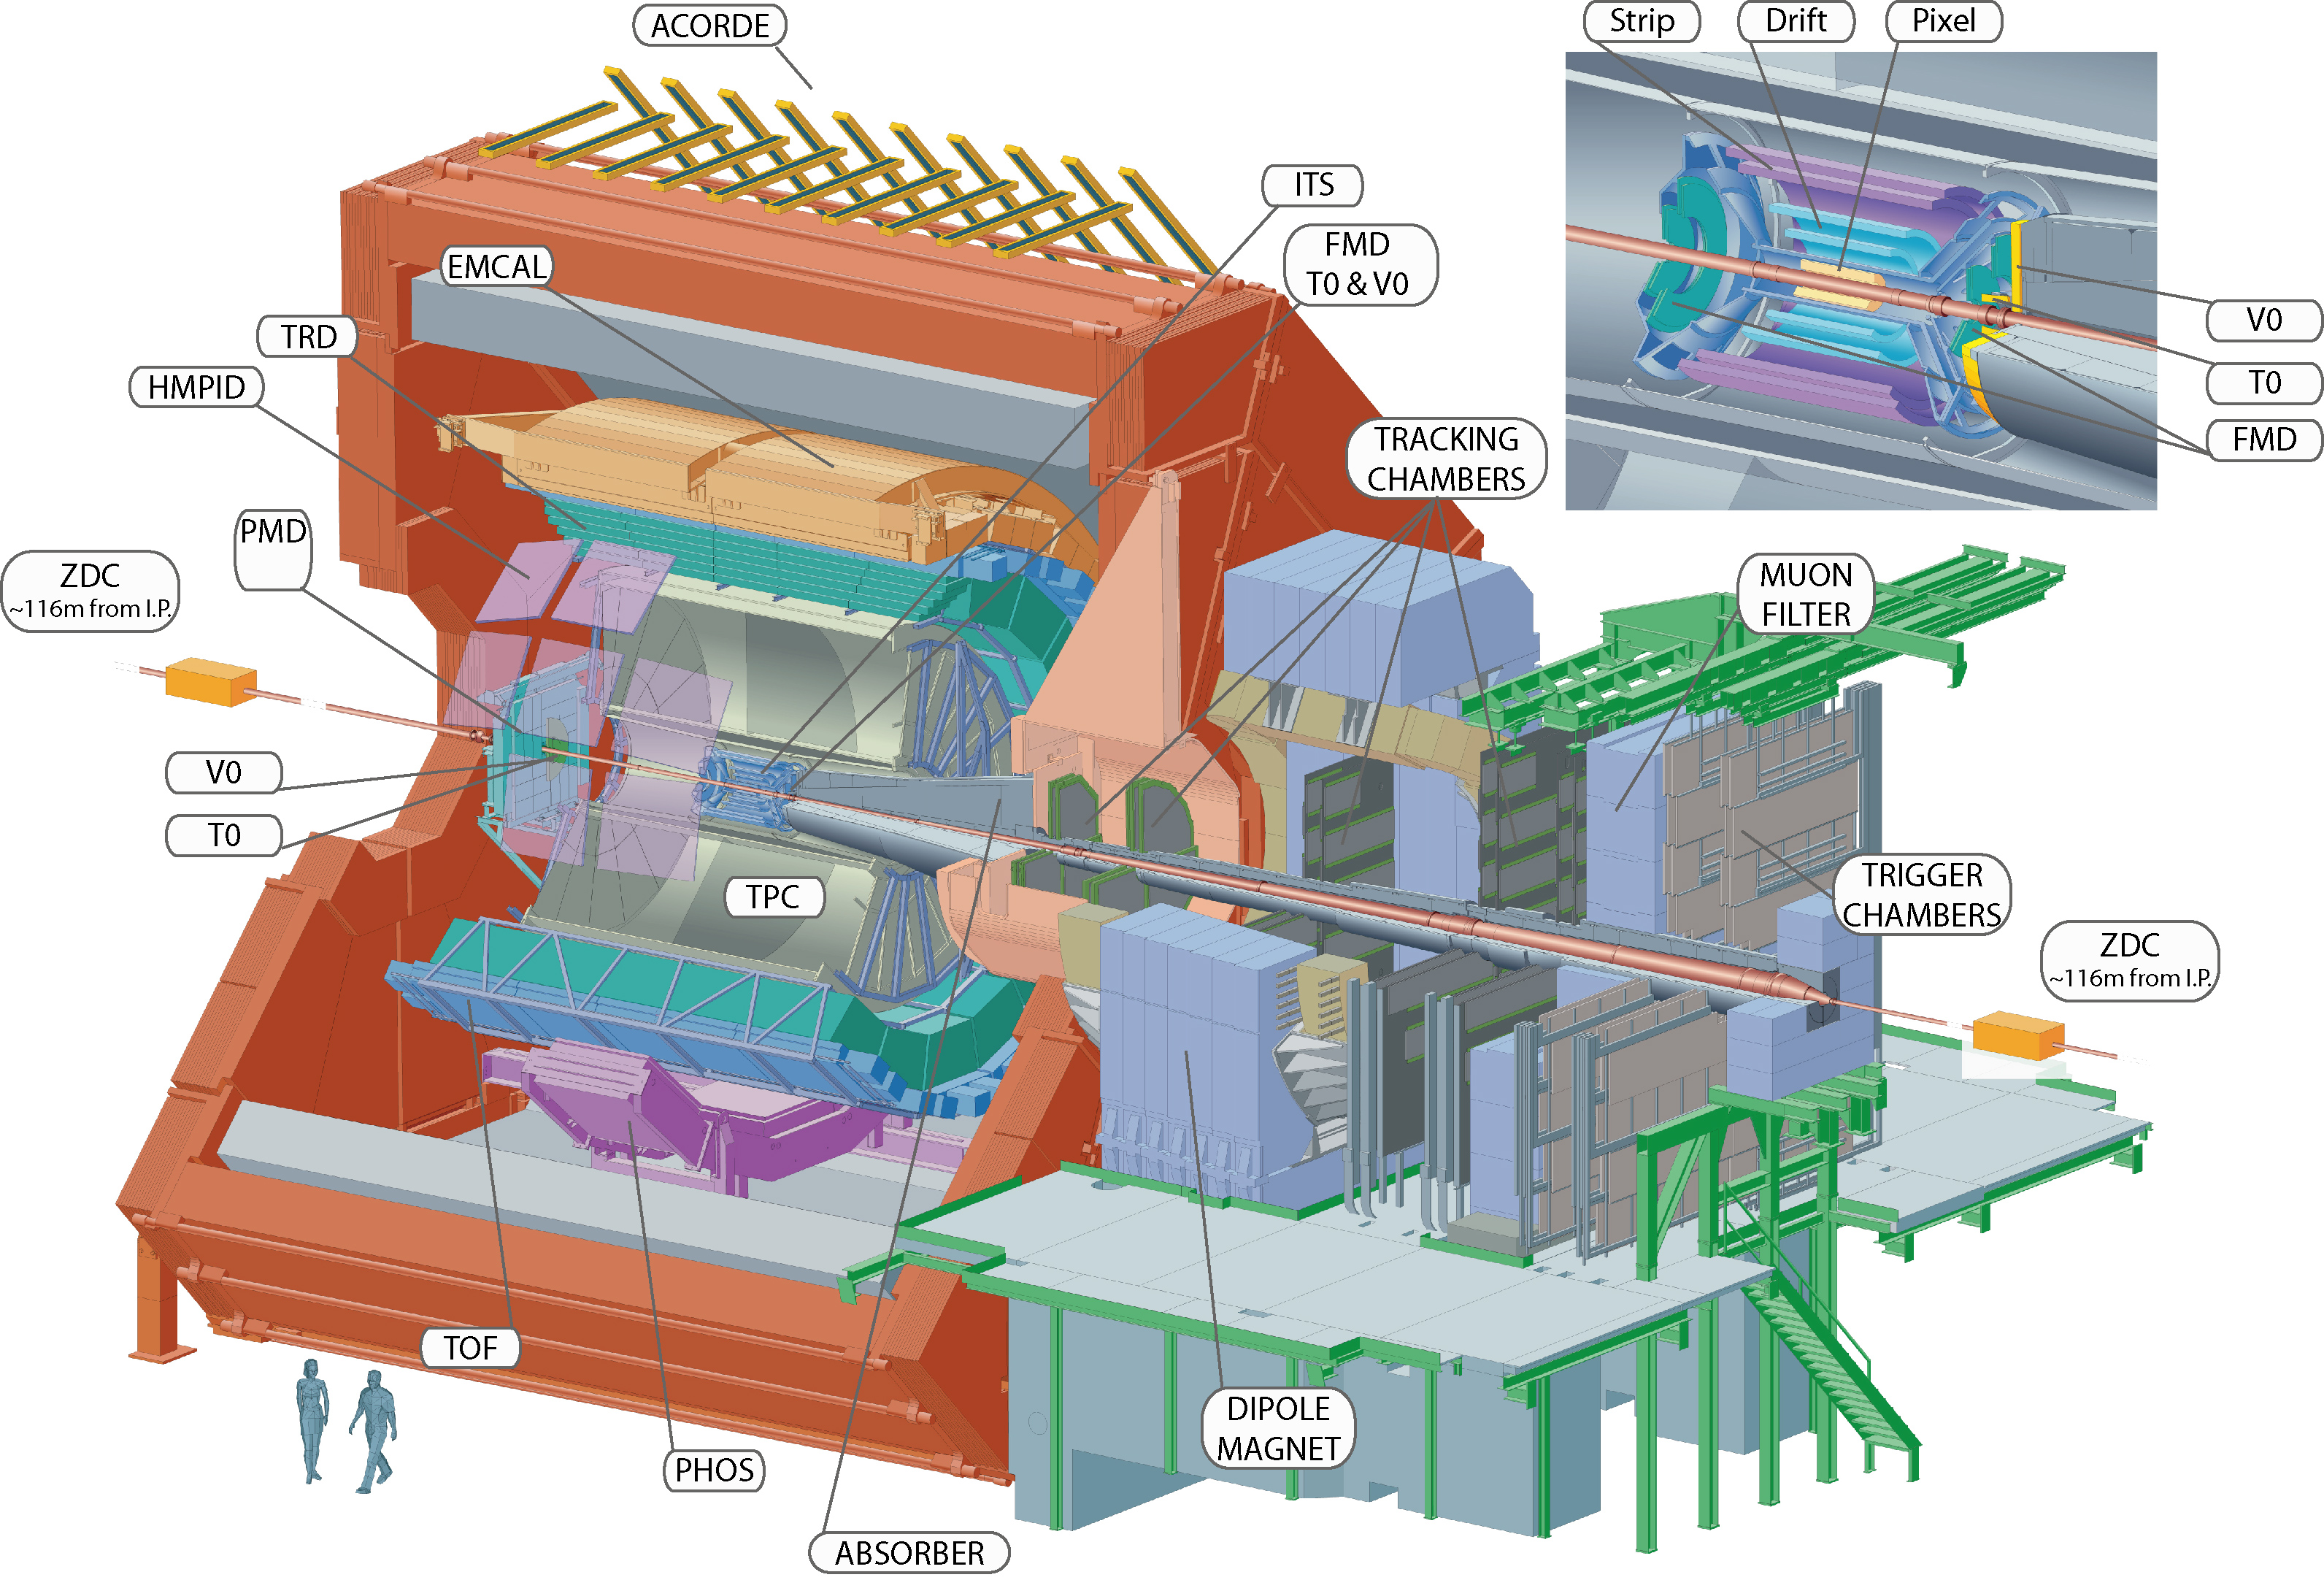
\includegraphics[width=\linewidth]{img/alice_schematics}
 \end{tikzfigure}
\end{minipage}
%
\begin{minipage}[t]{0.59\colwidth}
\begin{itemize}
\item Important features
\begin{itemize}
\item \textbf{Particle Identification} (PID) of
e, $\mu$, $\pi$, K, p, d, ${}^3$He
\item \textbf{low-momentum tracking} ($\pt > 0.15$~\GeVc)
\end{itemize}
\item \textbf{D mesons} via hadronic decays (ITS, TPC, TOF)
\begin{itemize}
\item PID, topological cuts on the decay products
\item invariant mass analysis
\end{itemize}
\item \textbf{Jet reconstruction} using \antikt\ algorithm
\begin{itemize}
\item \textcolor{ForestGreen}{charged constituents} (ITS, TPC) $\rightarrow$ \emph{charged jets}
\item add \textcolor{NavyBlue}{neutral constituents} (EMCal, DCal) $\rightarrow$ \emph{full jets} 
\end{itemize}
\end{itemize}
\end{minipage}
}
\end{columns}

\begin{columns}
\column{.55}
\block{Results: \Dzero-Jet \pt-Differential Cross Section}{
\begin{minipage}[t]{0.61\colwidth}
\vspace{-30pt}
\begin{tikzfigure}[Prompt \Dzero-jet \pt-differential cross section in \pp\ collisions at $\s=7$~TeV.\par]
     \label{fig:D0JetCrossSection_pp7TeV}
    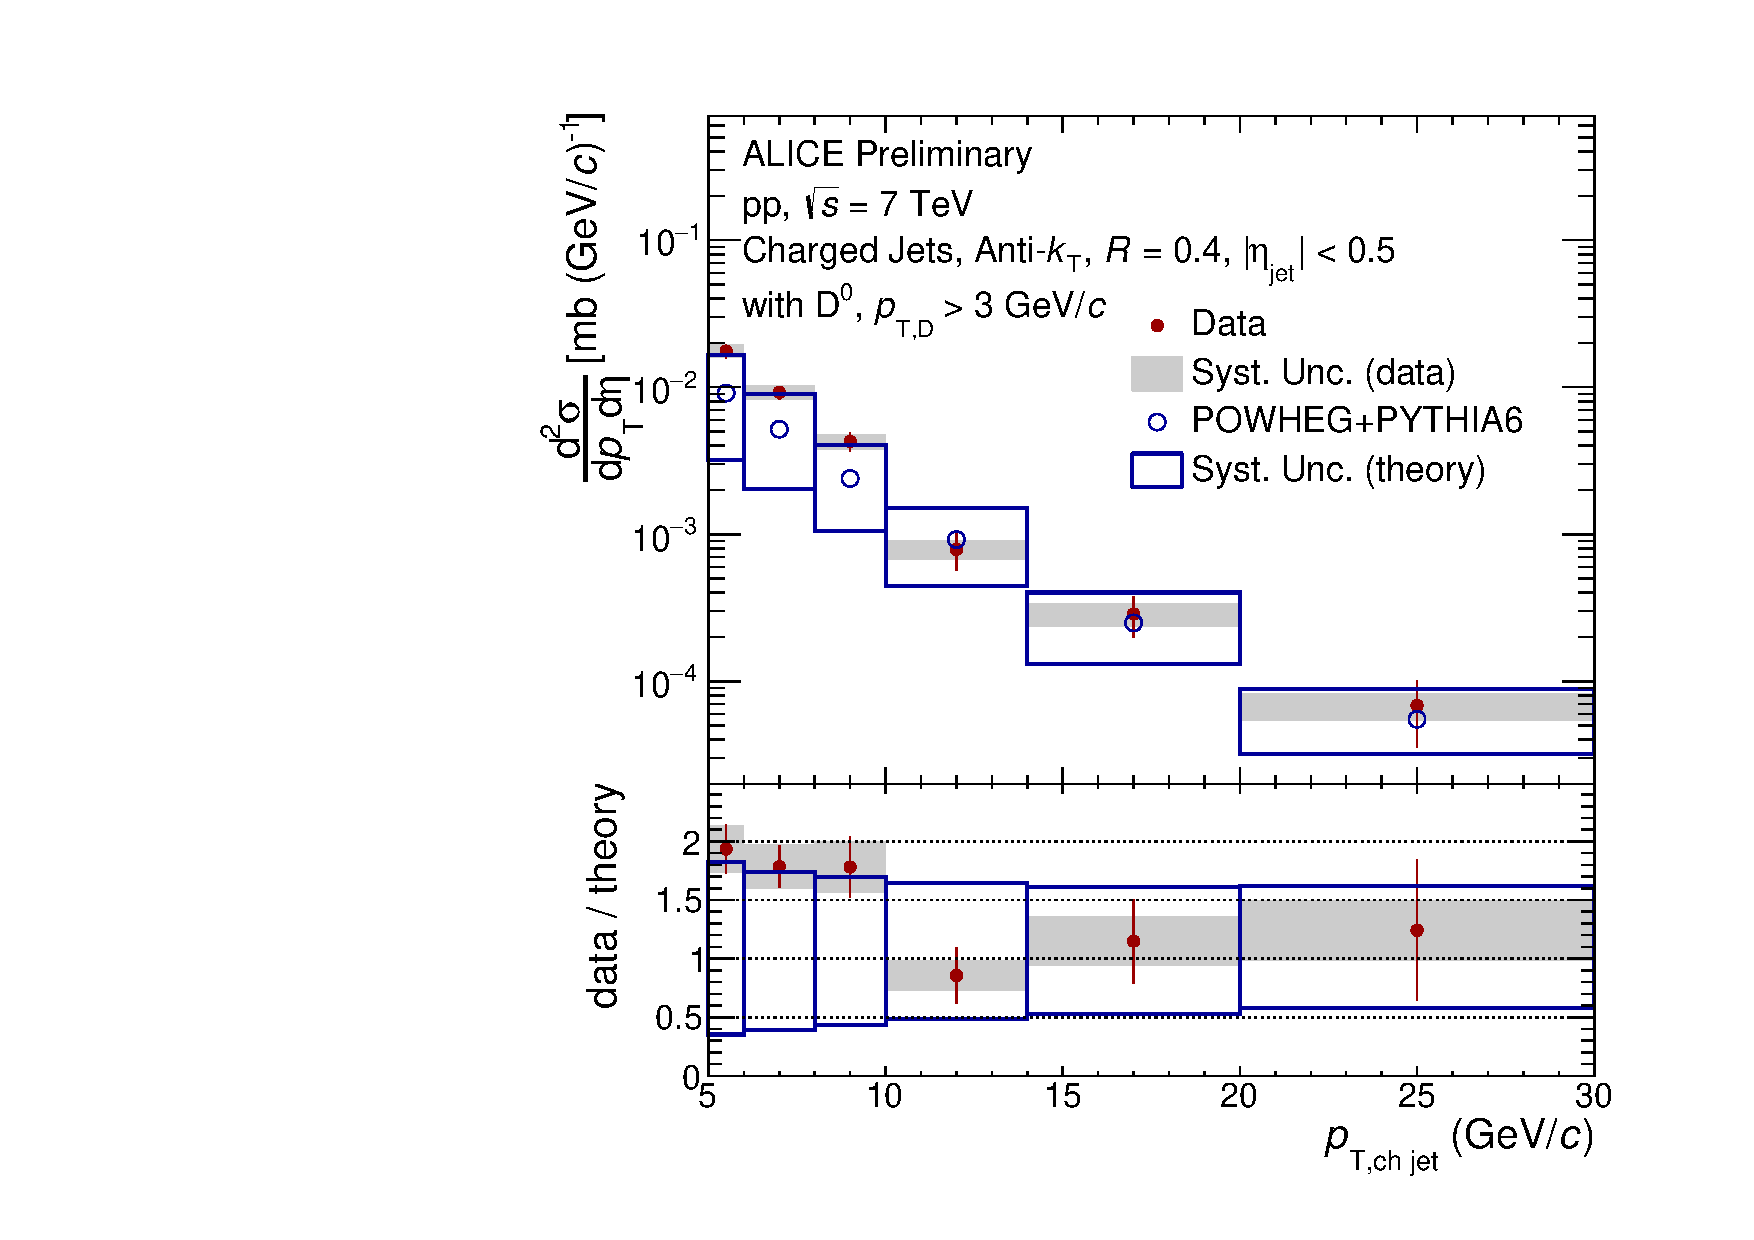
\includegraphics[width=1.07\linewidth]{img/D0JetCrossSection_pp7TeV}
 \end{tikzfigure}
\end{minipage}
%
\begin{minipage}[t]{0.34\colwidth}
\vspace{10pt}
\begin{itemize}
\item \textbf{\pp\ collisions at $\s=7$~TeV}
\item 355 M of minimum-bias events corresponding to $L_{\rm int}=5.7\, {\rm nb}^{-1}$
\item \Antikt\ jet finding algorithm
\item Charged constituents, $R=0.4$
\item Charm content tagged with \Dzero\
\item B feed-down subtracted using \\POWHEG+PYTHIA6
\item Corrected to particle level
\end{itemize}
Comparison with prediction from a \\Monte Carlo generator
\begin{itemize}
\item Parton event generator:\\ \textbf{POWHEG}
\item Shower and hadronization:\\ \textbf{PYTHIA6 (Perugia-2011)}
\end{itemize}
The data is in \textbf{good agreement} with the MC simulation,
although for $\ptchjet<10$~\GeVc\ data points lie at the edge of the uncertainty.
\end{minipage}
}
\column{.45}

\block{Raw Signal Extraction}{
\vspace{-30pt}
\begin{tikzfigure}[Top: invariant mass distributions; bottom: jet \pt\ distributions from signal region and side bands.\par]
     \label{fig:SideBandInvMass_QM17}
    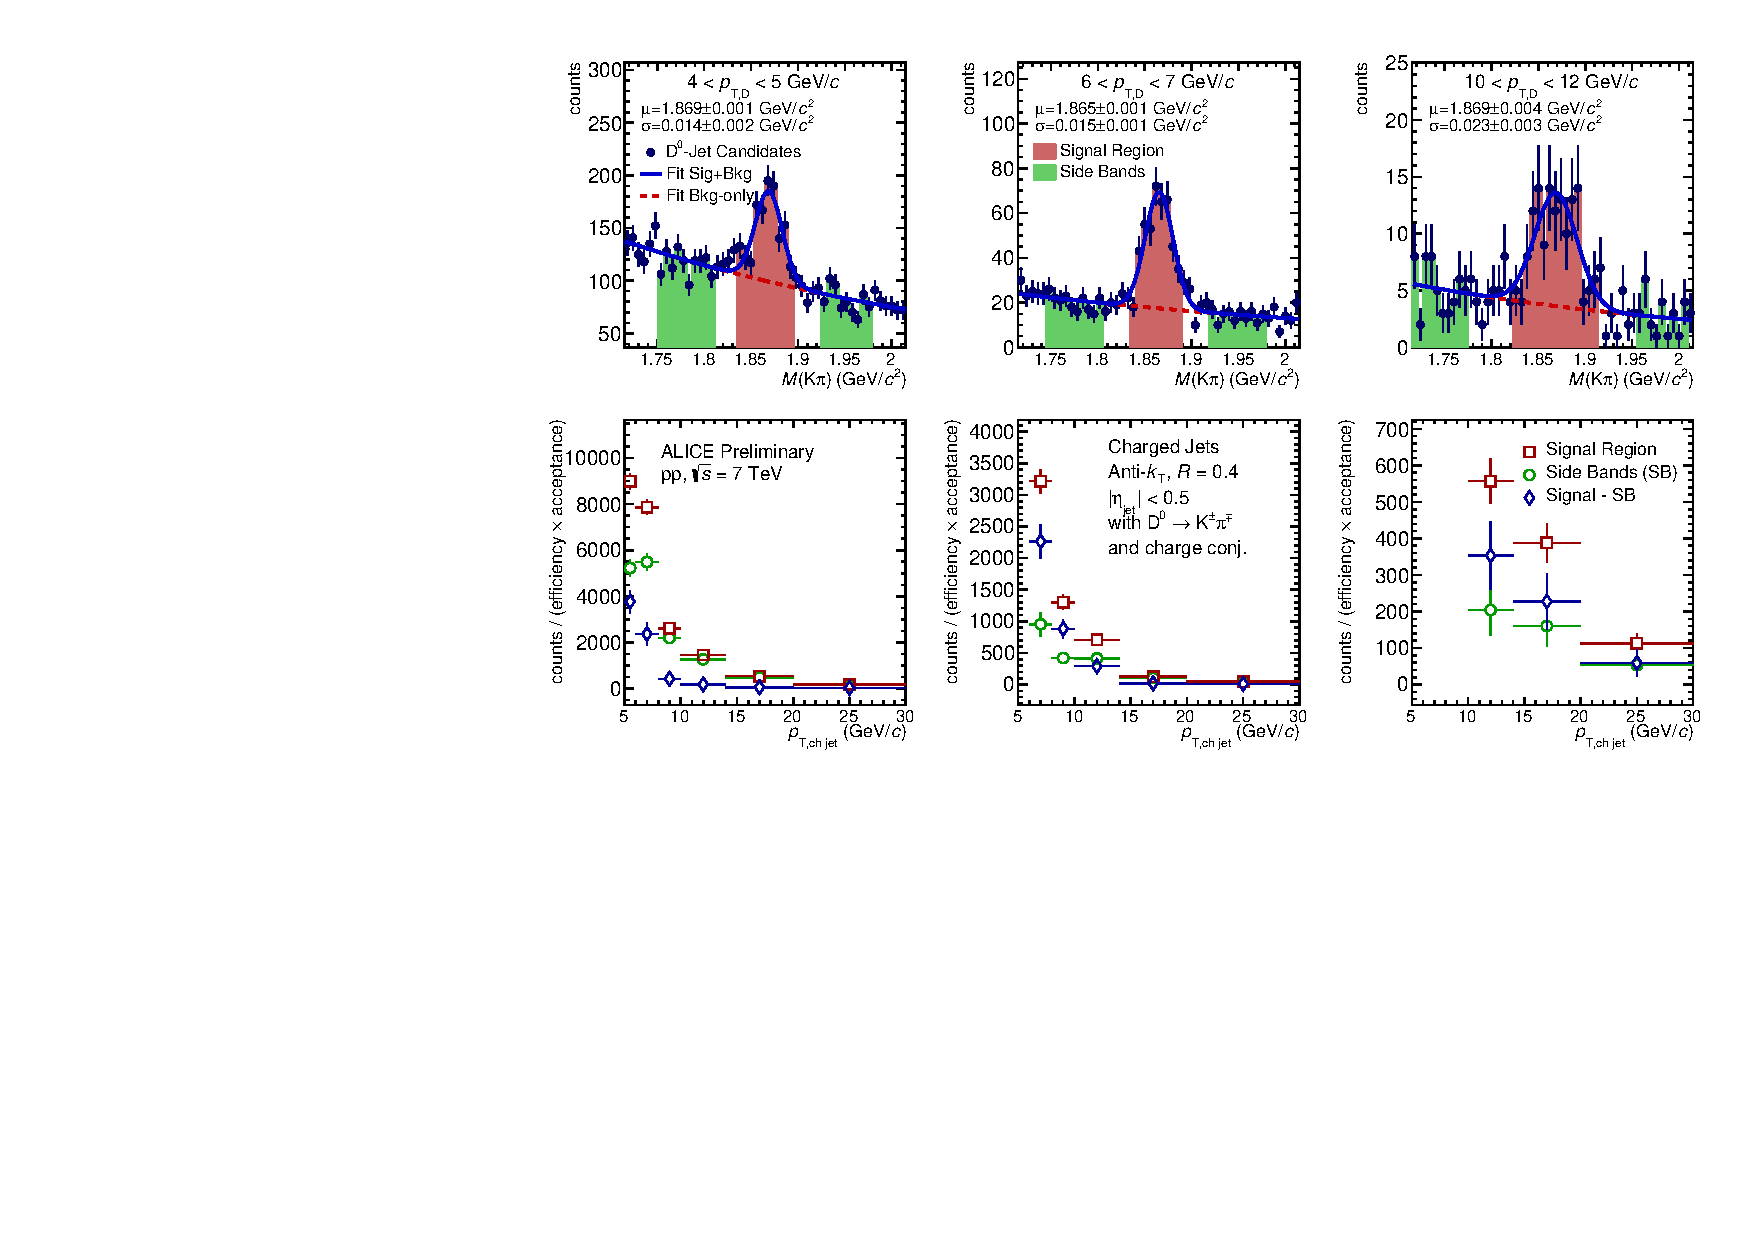
\includegraphics[width=.83\colwidth]{img/SideBandInvMass_QM17}
 \end{tikzfigure}
\begin{itemize}
\item \Dzero-candidate + all other charged tracks $\xrightarrow{\Antikt}$ \Dzero-jet candidate
\item The \textbf{\textcolor{darkestblue}{invariant mass distributions}} of identified \Dzero-jet candidates are\\ \textbf{\textcolor{darkblue}{fit}} in bins of \ptd\ to extract the peak position and width and the\\ background normalization $B'$
\item The \ptchjet\ distributions of the \textbf{\textcolor{lightgreen}{side bands}} are subtracted from those of the \textbf{\textcolor{lightred}{signal region}} and weighted by the efficiency $\epsilon_{\Dzero}(\ptd)$ % (Fig.~\ref{fig:HQ16_Simulation_EfficiencyVsDP})
\end{itemize}
\centering
 $\textcolor{darkerblue}{N(\ptchjet)}=\sum_{\ptd}\frac{1}{\epsilon_{\Dzero}(\ptd)} \cdot \left[\textcolor{lightred}{N_{\rm Sign}(\ptd,\ptchjet)}-B'\textcolor{lightgreen}{N_{\rm SB}(\ptd,\ptchjet)} \right]$
}
\end{columns}

\begin{columns}

\column{.38}
\block{Detector Performance}{
\begin{minipage}[t]{0.47\colwidth}
\begin{tikzfigure}[Mean and median of the JES shift.\par]
     \label{fig:HQ16_Simulation_EnergyScaleShift}
    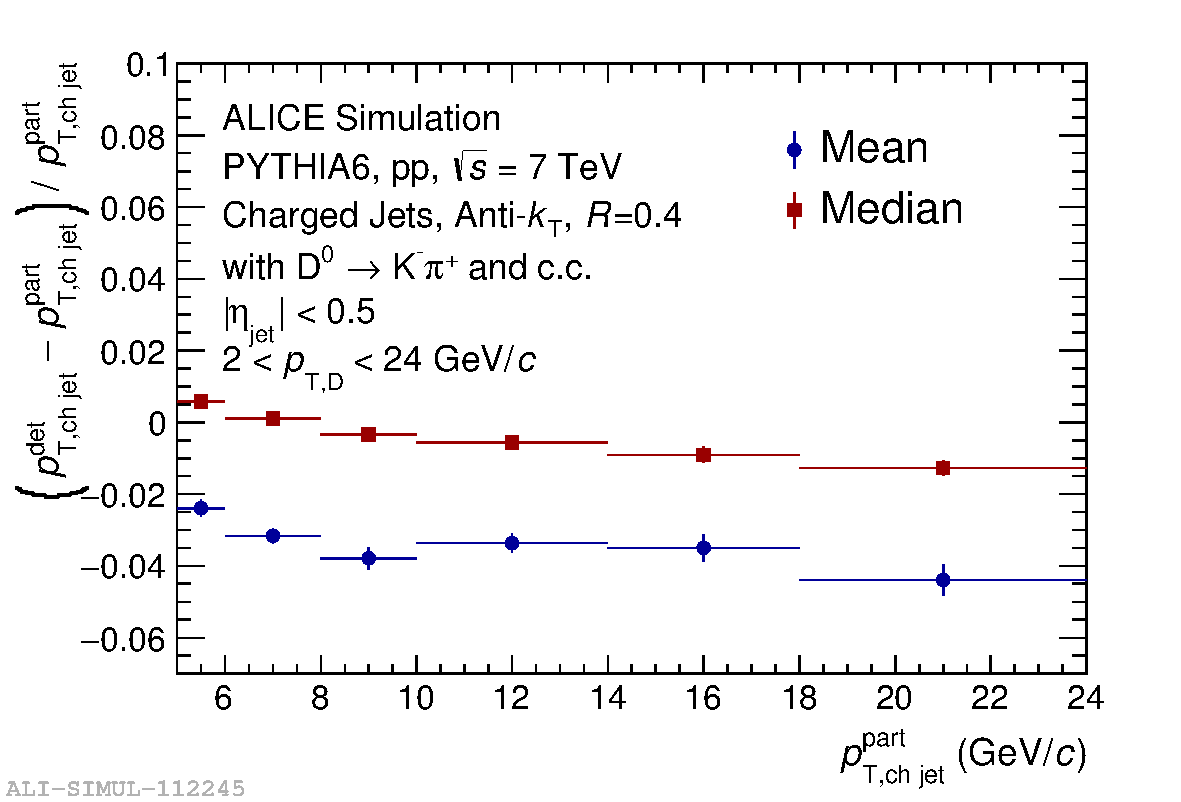
\includegraphics[width=.95\linewidth]{img/HQ16_Simulation_EnergyScaleShift}
 \end{tikzfigure}
\begin{tikzfigure}[Momentum shift distribution.\par]
     \label{fig:HQ16_Simulation_DetectorResponse}
    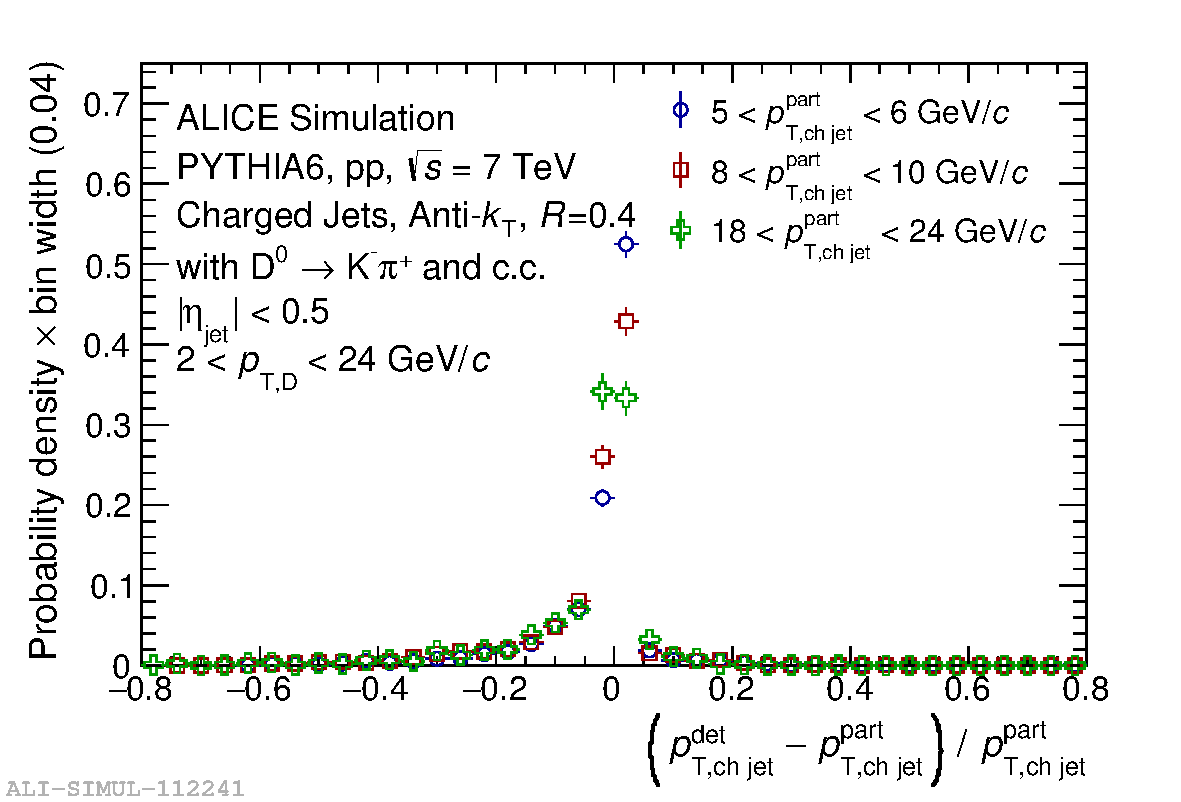
\includegraphics[width=.95\linewidth]{img/HQ16_Simulation_DetectorResponse}
 \end{tikzfigure}
\begin{tikzfigure}[Efficiency vs. \ptchjet.\par]
     \label{fig:HQ16_Simulation_EfficiencyVsDPt}
    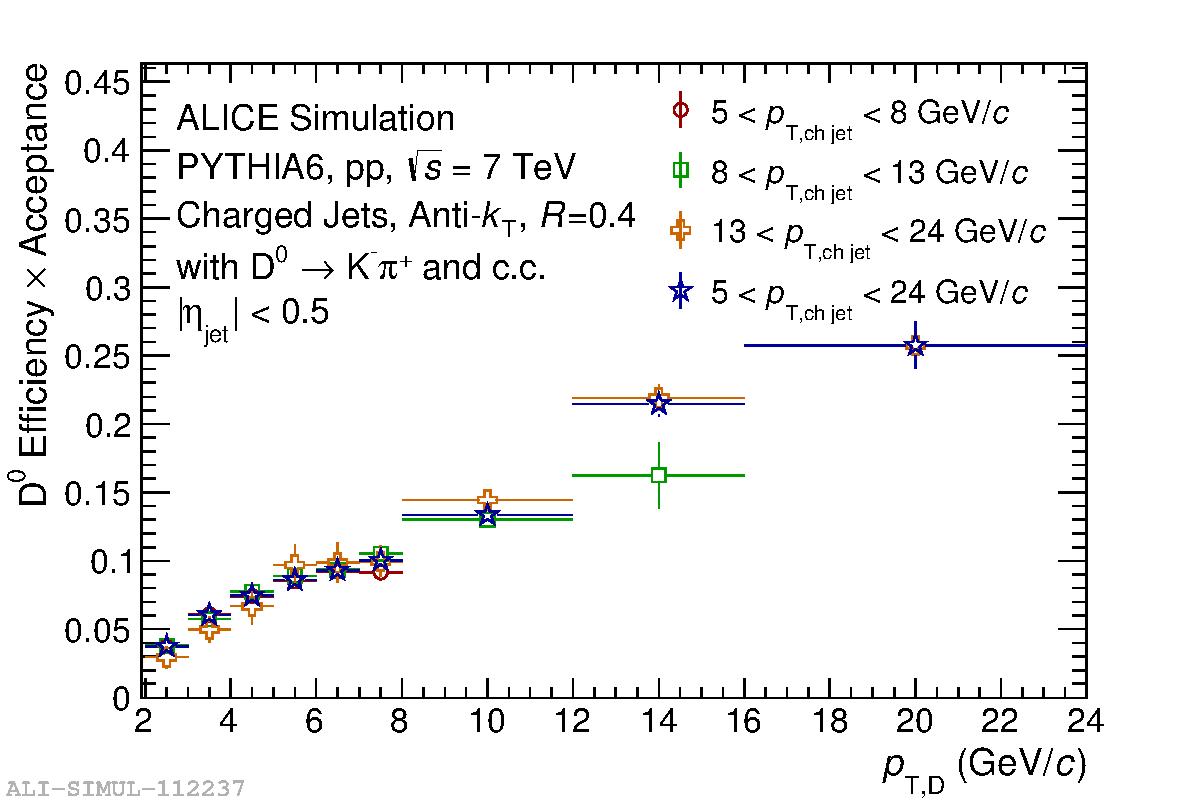
\includegraphics[width=.95\linewidth]{img/HQ16_Simulation_EfficiencyVsDPt}
 \end{tikzfigure}
\end{minipage}%
%
\begin{minipage}[t]{0.4465\colwidth}
\begin{tikzfigure}[Jet momentum resolution.\par]
     \label{fig:HQ16_Simulation_Resolution}
    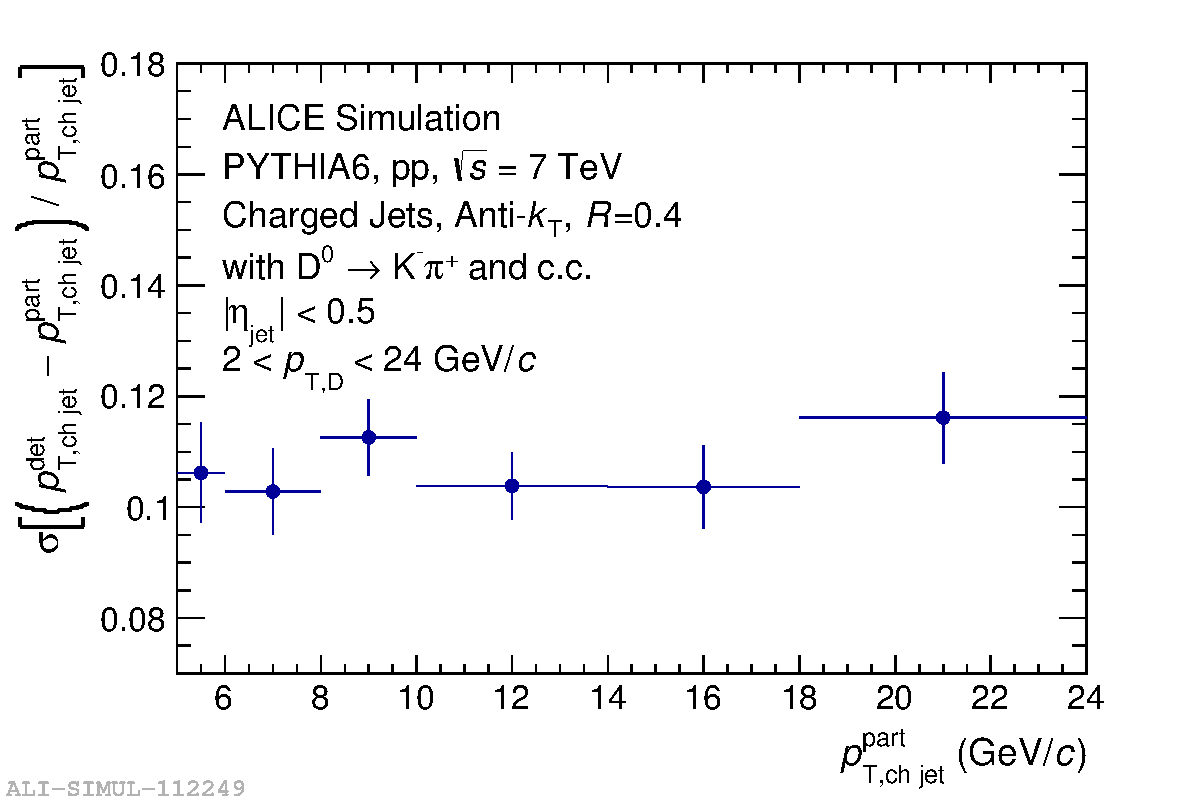
\includegraphics[width=\linewidth]{img/HQ16_Simulation_Resolution}
 \end{tikzfigure}
\vspace{25pt}
\begin{itemize}
\item PYTHIA6+GEANT3
\item Mean jet energy scale (JES) shift $\approx-3$~\%
\item Jet \pt\ resolution $\approx11$~\%,\\ independent of \ptchjet
\item The distribution of the momentum shift features a sharp peak at $0$ with a longer tail at negative values (expected due to tracking inefficiency)
\item The \Dzero\ reconstruction efficiency has weak or no dependence on the jet \pt\ $\rightarrow$ simplifies corrections and reduces systematics
\end{itemize}
\end{minipage}
}

\column{.62}


\block{B Feed-Down Subtraction}{
\begin{minipage}[t]{0.34\colwidth}
\hspace{20pt}
\begin{description}
\item[Prompt:]\hspace{2pt} fragmentation of a c quark 
\item[Non-Prompt:]\hspace{2pt} decay of a B meson
\end{description}
Due to the longer decay length of the B mesons, the topological cuts are more efficient for non-prompt \Dzero, thus biasing the
relative contributions. We subtract the B feed-down fraction using POWHEG+PYTHIA6.
\end{minipage}
%
\begin{minipage}[t]{0.30\colwidth}
\begin{tikzfigure}[Reconstruction efficiency.\par]
     \label{fig:Efficiency_QM17}
    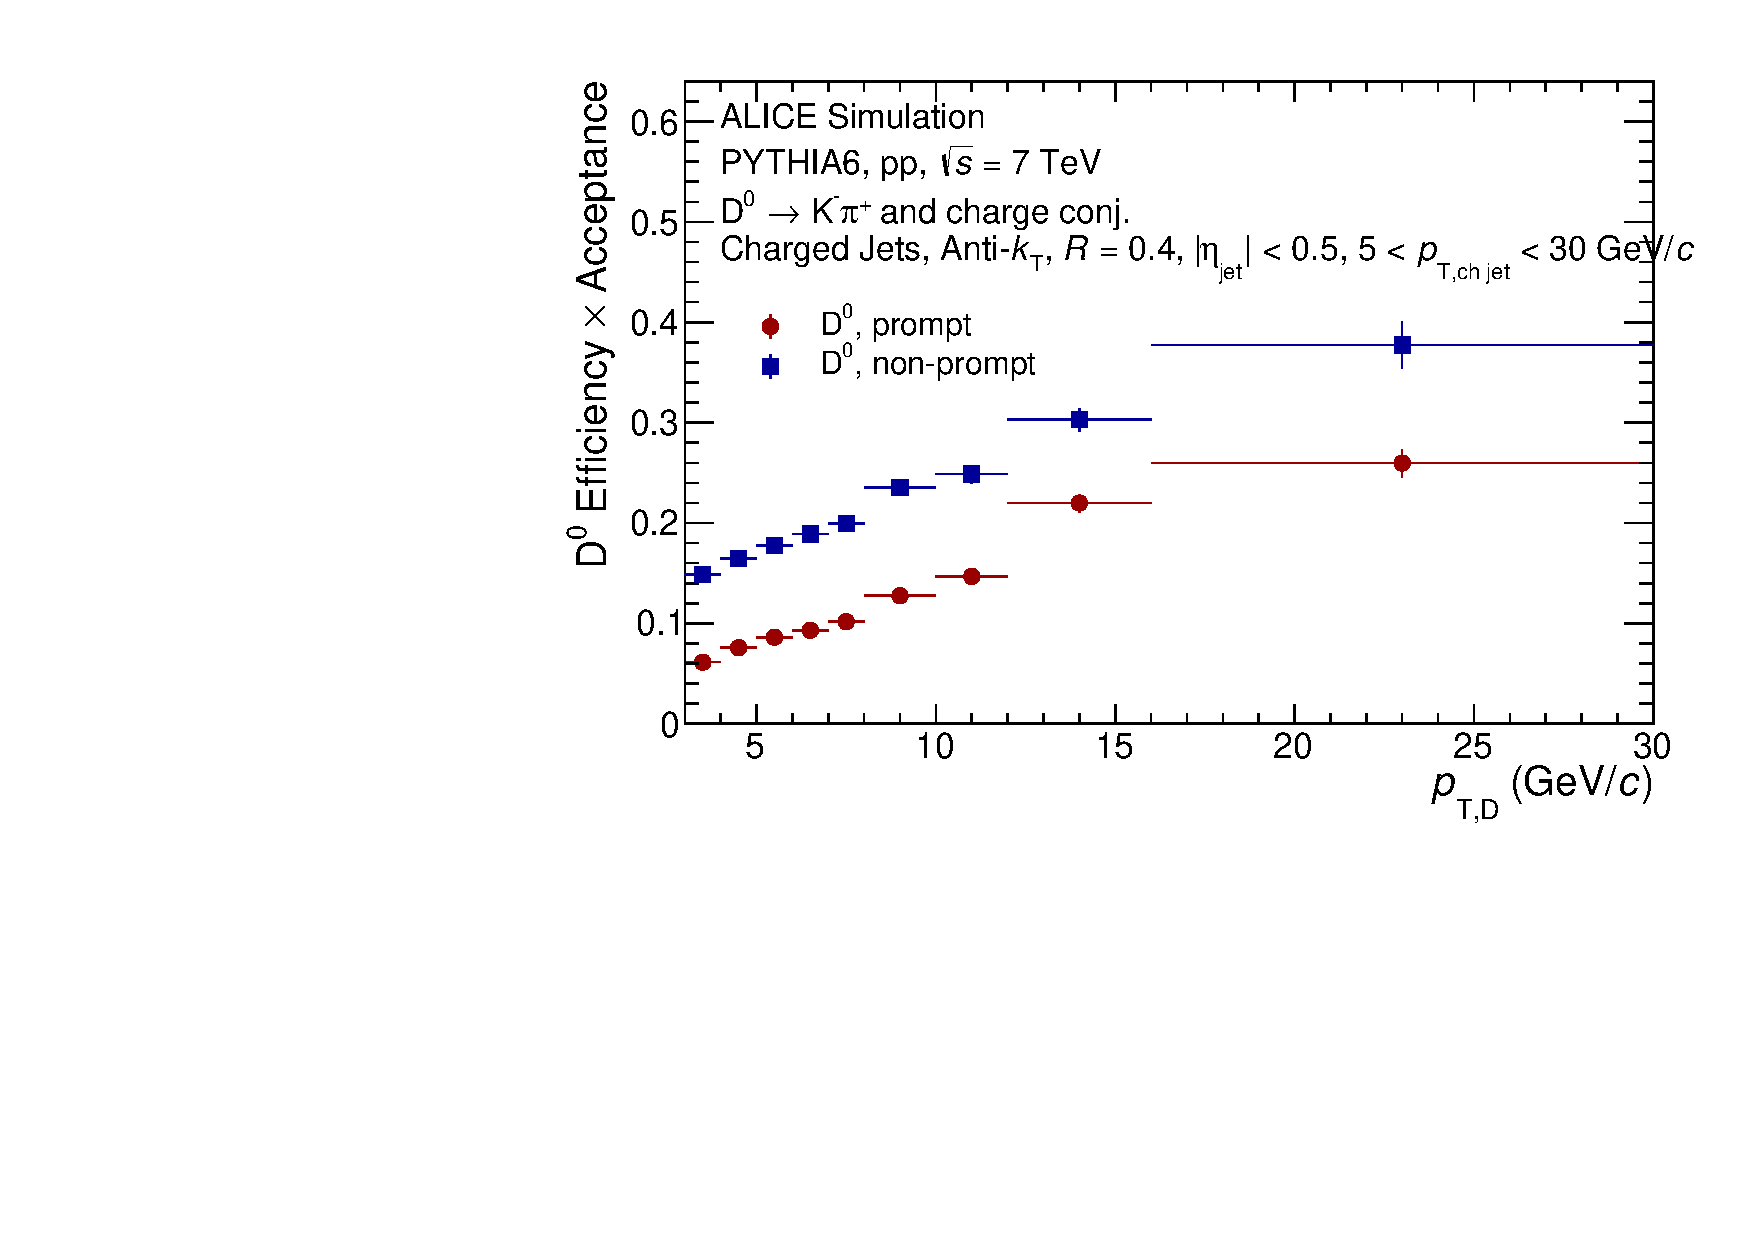
\includegraphics[width=\linewidth]{img/Efficiency_QM17}
 \end{tikzfigure} 
\end{minipage}
%
\begin{minipage}[t]{0.30\colwidth}
\begin{tikzfigure}[B feed-down fraction.\par]
     \label{fig:BFeedDown_QM17}
    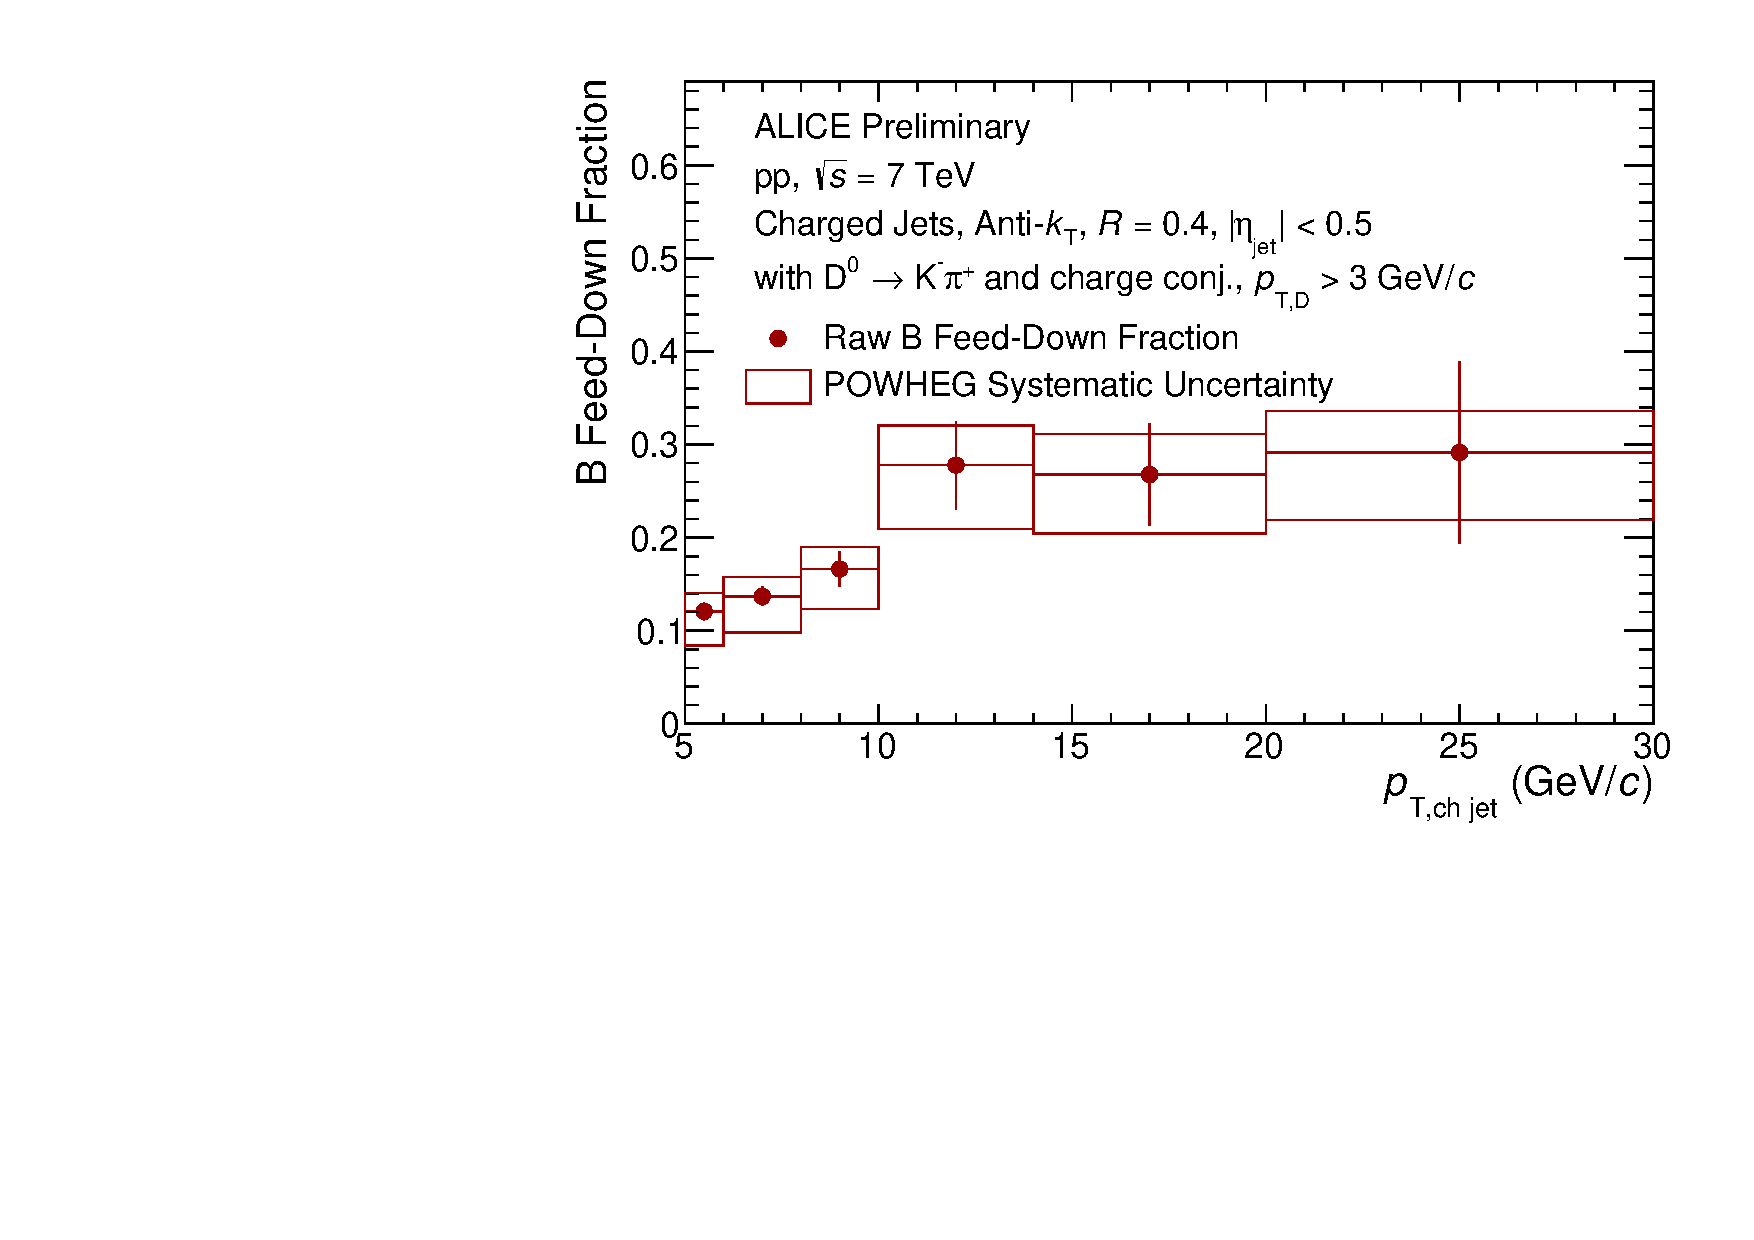
\includegraphics[width=\linewidth]{img/BFeedDown_QM17}
 \end{tikzfigure}
\end{minipage}
}

\block{Conclusions and Outlook}{
\begin{minipage}[t]{0.42\colwidth}
\vspace{-30pt}
\begin{tikzfigure}[Relative uncertainties.\par]
     \label{fig:Uncertainties_QM17}
    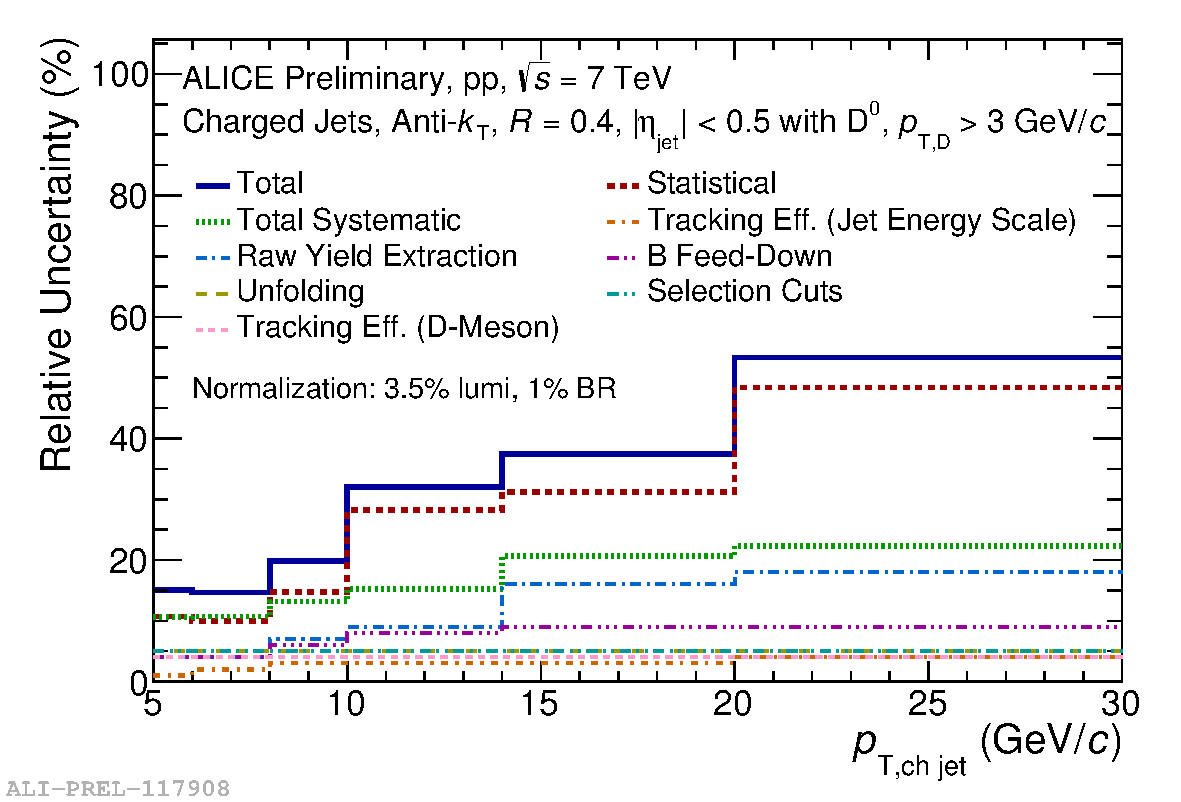
\includegraphics[width=\textwidth]{img/Uncertainties_QM17}
 \end{tikzfigure}
\end{minipage}
\begin{minipage}[t]{0.53\colwidth}
\begin{itemize}
\item ALICE has measured the cross section of charm (charged-only) jets tagged with \Dzero\ mesons in the range $5<\ptchjet<30$~\GeVc\ in \pp\ collisions at $\s=7$~TeV
\item POWHEG+PYTHIA6 is in \textcolor{ForestGreen}{\textbf{agreement with the data}}
\item Raw yield extraction is the larger systematic uncertainty, but \textcolor{BrickRed}{\textbf{precision of the measurement limited by statistics}}
\item In the near future we will extend this measurement to the larger datasets at $\s=8,13$~TeV using electromagnetic calorimeters for triggering and full jet reconstruction
\item The goal is the measurement of the \textcolor{NavyBlue}{\textbf{fragmentation of charm jets}} in an extended kinematic region
\end{itemize}
\end{minipage}
}

\end{columns}

\end{document}
